\chapter{Experimentación}

En este capítulo se expondrá la experimentación realizada para evaluar el agente propuesto.

Se empieza ofreciendo los detalles de la experimentación, centrándose en los parámetros utilizados y los experimentos a realizar. Tras esto, se muestran los resultados obtenidos por las dos familias de agentes propuestas (estándares y priorizadas), mostrando además los experimentos que llevaron a la elección del conjunto de datos. Finalmente, se realizará una comparativa de los mejores agentes de cada familia, comparando su rendimiento durante el entrenamiento y al enfrentarse a problemas nuevos, analizando los resultados obtenidos.

\section{Detalles de la experimentación}

En esta sección se describen los principales detalles de la experimentación: los \textbf{parámetros} a utilizar durante los experimentos, las \textbf{métricas} a medir y los \textbf{experimentos} que se ha optado por realizar.

\subsection{Parámetros generales utilizados}

Si bien hay algunos parámetros que varían entre experimentos, la gran mayoría de éstos son reutilizados por toda la experimentación. Para facilitar la reproducibilidad, estos parámetros serán descritos a continuación, mostrando sus valores y su significado.

Los parámetros utilizados y su origen se pueden observar en las siguientes tablas:
\begin{itemize}
	\item Parámetros usados por \textit{Deep Q-Learning} en el Cuadro \ref{tab:dqlparam}.
	
	Los parámetros están basados en los parámetros originales propuestos por DeepMind en su artículo original \cite{Mnih2015HumanlevelCT}, ajustados experimentalmente para adaptarse al problema.
	
	\item Parámetros usados durante el preprocesamiento de imágenes en el Cuadro \ref{tab:imageparam}.
	
	Los parámetros se han elegido manualmente mediante experimentación para ajustarse a las necesidades del problema.
	
	\item Parámetros usados durante la generación de las recompensas en el Cuadro \ref{tab:rewardparam}.
	
	Los parámetros están basados en los parámetros originales propuestos por Carlos Sampedro \textit{et al.} en su trabajo original \cite{Sampedro2018}, adaptándose de forma experimental a las necesidades del proyecto.
\end{itemize}

\begin{table}[h]
\centering
\resizebox{\textwidth}{!}{%
\begin{tabular}{@{}lll@{}}
\toprule
Hiperparámetro                                                                       & Valor & Descripción                                                                                                                                                      \\ \midrule
seed                                                                                 & 0     & Semilla usada para los experimentos                                                                                                                              \\
learning\_rate                                                                       & 0.001 & Ratio de aprendizaje de la red neuronal                                                                                                                          \\
gamma ($\gamma$)                                                                     & 0.99  & Ratio de aprendizaje de DQL                                                                                                                                      \\
epsilon ($\epsilon$)                                                                 & 1.00  & Probabilidad inicial de realizar una acción aleatoria                                                                                                            \\
min\_epsilon ($\epsilon_{min}$)                                                      & 0.05  & \begin{tabular}[c]{@{}l@{}}Probabilidad final de realizar una acción aleatoria\\ (tras min\_epsilon\_percentage episodios)\end{tabular}                          \\
\begin{tabular}[c]{@{}l@{}}min\_epsilon\_percentage \\ ($min\_epsilon$)\end{tabular} & 0.8   & \begin{tabular}[c]{@{}l@{}}Porcentaje de episodios tras el cual epsilon alcanza min\_epsilon\\ (tras el 80\% de los episodios alcanza min\_epsilon)\end{tabular} \\ \bottomrule
\end{tabular}%
}
\caption{Parámetros generales de \textit{Deep Q-Learning.}}
\label{tab:dqlparam}
\end{table}

\begin{table}[h]
\centering
\resizebox{\textwidth}{!}{%
\begin{tabular}{@{}lll@{}}
\toprule
Hiperparámetro      & Valor & Descripción                                                                                                                                                                          \\ \midrule
trim                & 35    & \begin{tabular}[c]{@{}l@{}}Número de píxeles recortados a la imagen por los\\ extremos inferior y superior\end{tabular}                                                              \\
obstacle\_threshold & 0.15  & \begin{tabular}[c]{@{}l@{}}Umbral en la cámara de profundidad a partir del cual\\ se consideran obstáculos\\ (los objetos a menos de obstacle\_threshold son obstáculos)\end{tabular} \\
min\_contour\_area  & 250   & \begin{tabular}[c]{@{}l@{}}Área mínima (en píxeles) de un contorno \\ para ser considerado obstáculo\end{tabular}                                                                    \\ \bottomrule
\end{tabular}%
}
\caption{Parámetros generales del procesamiento de imágenes.}
\label{tab:imageparam}
\end{table}

\begin{table}[h]
\centering
\resizebox{\textwidth}{!}{%
\begin{tabular}{@{}lll@{}}
\toprule
Hiperparámetro                                                                     & Valor & Descripción                                                                                                                                                                                                      \\ \midrule
obstacle\_distance ($l_{max}$)                                                     & 2     & \begin{tabular}[c]{@{}l@{}}Distancia aproximada (en metros) a la que se encuentra un\\ obstáculo en el umbral de detección\end{tabular}                                                                          \\
attraction\_gain ($\alpha$)                                                        & 100   & Ganancia aplicada a la fuerza atractora para aumentar su influencia                                                                                                                                              \\
repulsive\_gain ($\beta$)                                                          & 15    & Ganancia aplicada a la fuerza repulsiva para aumentar su influencia                                                                                                                                              \\
repulsive\_limit ($k$)                                                             & 0.04  & Valor usado para limitar la influencia de la fuerza repulsiva                                                                                                                                                    \\
\begin{tabular}[c]{@{}l@{}}repulsive\_goal\_influence \\ ($d_{infl}$)\end{tabular} & 0.75  & \begin{tabular}[c]{@{}l@{}}Porcentaje usado para limitar la influencia de la fuerza repulsiva\\ Si la distancia a la meta es menor que $l_{max} * d_{infl}$,\\ la fuerza repulsiva se ve disminuida\end{tabular} \\
success\_reward                                                                    & 10    & Recompensa por un episodio con éxito                                                                                                                                                                             \\
failure\_penalty                                                                   & -100  & Penalización por un episodio fallido o una colisión                                                                                                                                                              \\ \bottomrule
\end{tabular}%
}
\caption{Parámetros generales de la generación de recompensas.}
\label{tab:rewardparam}
\end{table}

Los parámetros específicos usados por cada experimento serán detallados durante la definición de los experimentos a realizar. La lista concreta y completa de los parámetros de cada experimento está disponible en el fichero de configuración correspondiente.

\subsection{Experimentos realizados}

Se ha optado por realizar un total de \textbf{ocho} experimentos, diviendo estos experimentos en dos grandes grupos:

\begin{itemize}
	\item \textbf{Entrenamiento de agentes estándares:} Estos experimentos consisten en el entrenamiento de agentes utilizando una versión estándar de \textbf{Deep Q-Learning} (sin ninguna de las mejoras propuestas) durante un total de \textbf{15000} episodios. Estos agentes cuentan con un \textit{Replay Memory} de \textbf{20000} entradas, usando muestras de \textbf{64} experiencias por entrenamiento.
	
	Especificamente, se han entrenado las siguientes combinaciones de parámetros:
	\begin{itemize}
		\item Recompensa de contornos / Sin colisiones.
		\item Recompensa de contornos / Con colisiones.
		\item Recompensa de columnas (8 columnas) / Sin colisiones.
		\item Recompensa de columnas (8 columnas) / Con colisiones.
	\end{itemize}
	
	\item \textbf{Entrenamiento de agentes priorizados:} Estos experimentos consisten en el entrenamiento de agentes utilizando \textbf{Deep Q-Learning} con \textbf{Prioritized Experience Replay} (muestreando las experiencias con más error) durante un total de \textbf{3000} episodios. Estos agentes cuentan con un \textit{Replay Memory} de \textbf{5000} entradas, usando muestras de \textbf{32} experiencias por entrenamiento. Además, \textit{Prioritized Experience Replay} utiliza parámetros $\alpha = 0.5$ y $\beta = 0.5$.
	
	Especificamente, se han entrenado las siguientes combinaciones de parámetros:
	\begin{itemize}
		\item Recompensa de contornos / Sin colisiones.
		\item Recompensa de contornos / Con colisiones.
		\item Recompensa de columnas (8 columnas) / Sin colisiones.
		\item Recompensa de columnas (8 columnas) / Con colisiones.
	\end{itemize}
	
	El motivo de que el entrenamiento de estos agentes haya sido más corto y limitado (a nivel de tamaño del \textit{Replay Memory}) es las limitaciones en la capacidad computacional disponible durante el entrenamiento. El algoritmo es notablemente más lento y requiere una mayor cantidad de memoria, por lo que fue necesario reducir la envergadura de los experimentos para permitir acabarlos en un tiempo razonable. 
\end{itemize}

Tras la experimentación de ambos grupos, se realizan comparaciones del rendimiento de los dos mejores agentes de cada grupo durante \textbf{3000} episodios, para compararlos en condiciones de igualdad. Finalmente, se comparará el rendimiento de todos los agentes junto a varios \textit{benchmarks} ofrecidos por \textit{Habitat} (incluyendo varios agentes aleatorios y heurísticos y un agente implementando \textit{Proximal Policy Optimization}) para estudiar el rendimiento de cada agente al enfrentarse a problemas reales.

Todos los experimentos han sido realizados usando el conjunto de datos \textit{Gibson}, al ser éste considerado un conjunto de datos más simple que \textit{Matterport3D} \cite{habitat19iccv}. Además, se ha realizado una experimentación breve (detallada en la próxima sección) que apoya esta decisión.

\subsection{Gráficos generados durante el entrenamiento}

Como ya se mencionó en el Capítulo 5, el proceso de entrenamiento del agente almacena las siguientes métricas en un fichero de \textit{log} al final de cada episodio:
\begin{itemize}
	\item Número del episodio.
	\item Duración del episodio (en segundos).
	\item Número de acciones realizadas durante el episodio.
	\item Distancia inicial y final hasta la meta.
	\item Distancia recorrida hasta la meta ($dist\_inicial - dist\_final$).
	\item Exitoso (\textbf{Verdadero} si el agente ha alcanzado la meta, \textbf{Falso} en cualquier otro caso).
	\item Recompensa media obtenida.
\end{itemize}

Ahora bien, no todas estas métricas son comparables de forma honesta. Por ejemplo, al tener cada episodio una distancia inicial distinta, la distancia recorrida no se puede comparar de forma directa. Por tanto, se ha optado por transformar algunas de las métricas para poder realizar una comparación más justa, generando los siguientes \textbf{gráficos} durante el entrenamiento:
\begin{itemize}
	\item Diagrama de lineas de la duración por episodio (en segundos).
	\item Diagrama de lineas de la duración cumulativa por episodio (en segundos).
	\item Diagrama de lineas de las acciones realizadas por episodio.
	\item Diagrama de lineas del \textbf{porcentaje de distancia recorrido} hasta la meta.
	
	Este porcentaje, en el rango $[0.0, 1.0]$, indica el porcentaje total de distancia recorrido desde la posición inicial hasta la meta. Como ejemplo, un agente con distancia inicial de $10$ metros y distancia final de $5$ metros tendría un porcentaje de $0.5$.
	
	Se utiliza un porcentaje para normalizar la distancia recorrida por cada agente, cambiando la unidad de metros (no indicativa debido a la variabilidad en la longitud total de los episodios) a un porcentaje indicando la cantidad de episodio completada.
	\item Diagrama de lineas de recompensa media por episodio.
	\item Diagrama de barras del \textbf{número total de episodios completados con éxito}.
	
	Este diagrama permite comparar el rendimiento de los agentes de forma más simple que intentar interpretar el diagrama de distancias para observar los episodios completados.
\end{itemize}

Todos los diagramas de lineas han sido \textbf{suavizados} usando como datos la \textbf{media de los valores de los 50 episodios}. De esta forma se reduce notablemente el ruido en las gráficas (haciendolos más legibles) sin perder la información recogida en éstos.

\subsubsection{Métricas usadas durante la evaluación}

Para la evaluación del rendimiento de los agentes entrenados, se mide el valor medio de las siguientes métricas durante \textbf{100} episodios en entornos no usados durante el entrenamiento:
\begin{itemize}
	\item Distancia a la meta (en metros).
	\item Tasa de éxito.
	\item \textit{Success weighted by Path Length (SPL)}.
	\item \textit{SPL} suavizado.
	\item Número de colisiones.
\end{itemize}

Además, se ofrecen vídeos mostrando el rendimiento de los agentes en los entornos, para poder observar de forma directa el comportamiento de los agentes entrenados.

\section{Resultados obtenidos}

En esta sección se muestran los resultados obtenidos para cada grupo de experimentos mencionado previamente. Además, se muestra un breve análisis de los resultados que propiciaron elegir \textit{Gibson} como conjunto de datos.

\subsection{Elección del conjunto de datos}

Para estudiar la elección del conjunto de datos, se ha comparado el rendimiento de dos agentes equivalentes (\textit{Deep Q-Learning} básico sin colisiones con recompensas de contornos) durante \textbf{15000} episodios de entrenamiento, con especial interés en los episodios completados con éxito y la distancia recorrida hasta la meta.

\begin{figure}[h]
    \centering
    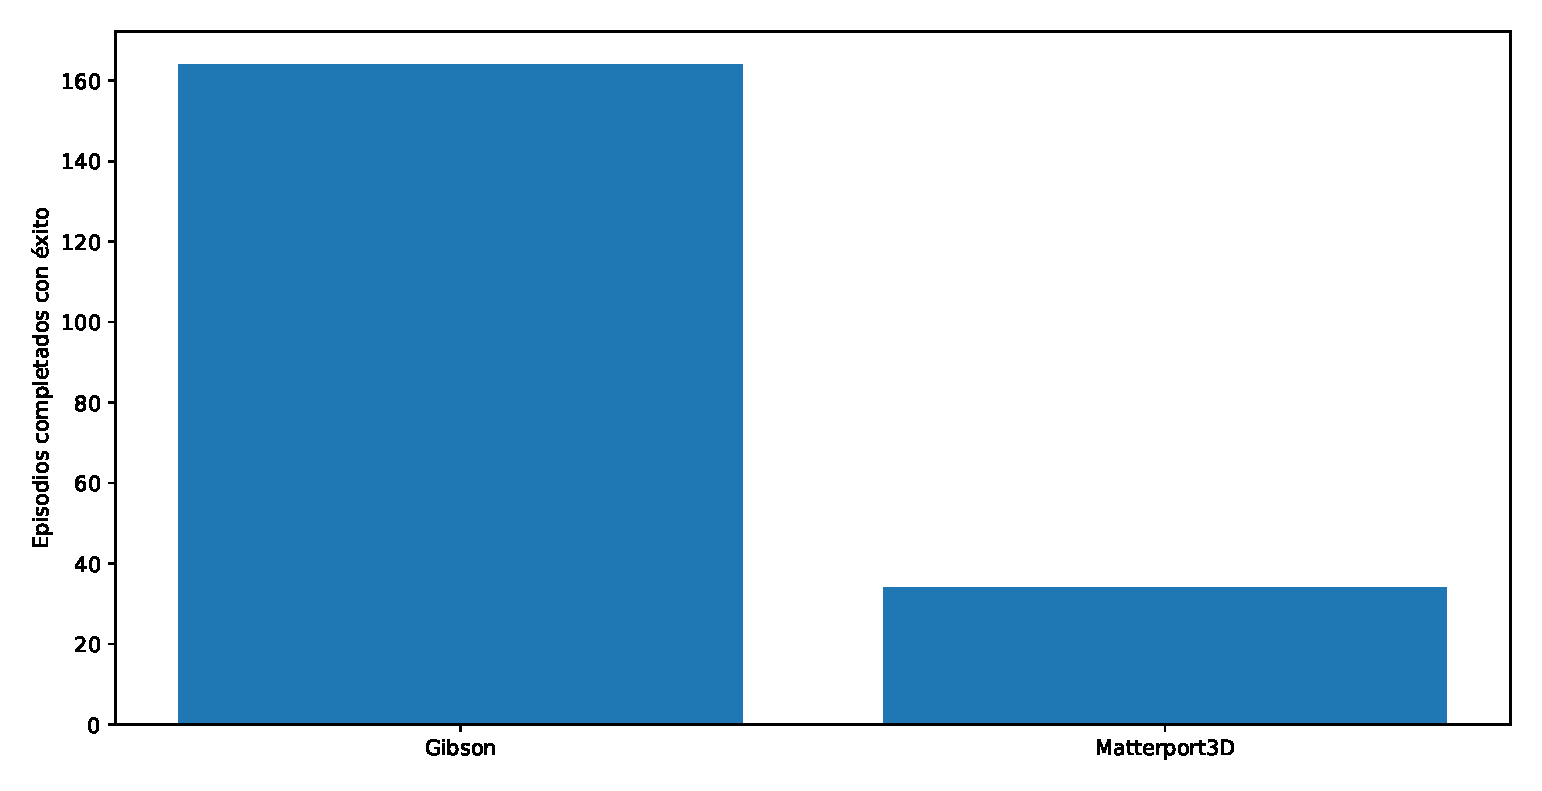
\includegraphics[width=\textwidth]{imagenes/cap6/dataset/success.eps}
    \caption{Comparativa de episodios completados con éxito entre conjuntos de datos.}
    \label{fig:chap6-dataset-success}
\end{figure}

\subsection{Agentes con \textit{Deep Q-Learning} estándar}

\subsection{Agentes con \textit{Deep Q-Learning} priorizado}

\section{Comparativa y análisis de resultados}

\subsection{Comparativa durante el entrenamiento}

\subsection{Comparativa durante la evaluación}
[TASA DE EXITO, CUAL ES MEJOR, ETC]

\subsection{Análisis de los resultados}